\section{Le plan de feu}
\label{sec:plan_de_feu}

Le plan de feu est un document essentiel pour la préparation d'un spectacle lumière.
Il s'agit d'un plan de la scène sur lequel sont indiqués l'emplacement de chaque projecteur, ecran ou autre élément lumineux.
Le plan de feu est réalisé sur un logiciel dédié, tel que Capture ou Wysiwyg. Non seulement il permet de placer les projecteurs, mais aussi de simuler leur rendu dans un environnement 3D.
On peut aussi connecter le logiciel à la console pour simuler la programmation en direct.
\newline
Le présent manuel n'a pas pour but de détailler la réalisation d'un plan de feu, mais il est important de savoir que ce document est essentiel pour la programmation lumière.
En voici un exemple ci-dessous, réalisé sur le logiciel Wysiwyg.

\begin{figure}[h]
    \centering
    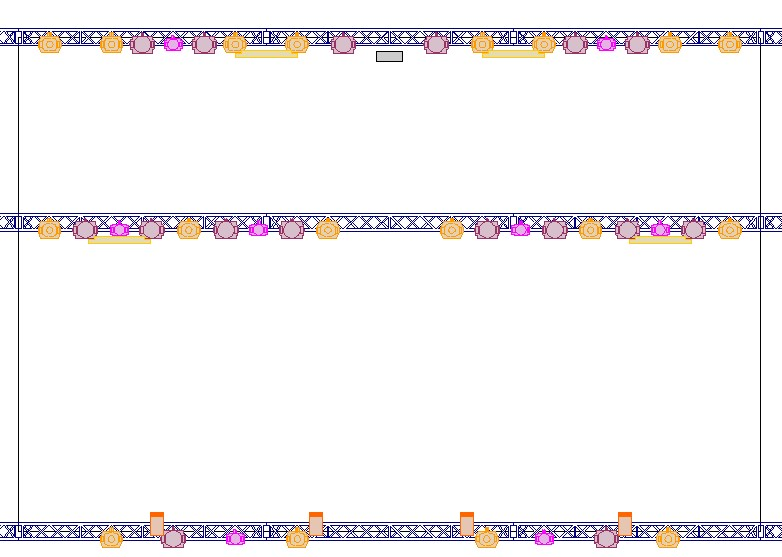
\includegraphics[width=0.8\textwidth]{2 - Généralités/Images/plan_de_feu.jpg}
    \caption{Exemple de plan de feu - Soirée Des Finaux P24}
    \label{fig:plan_de_feu}
\end{figure}
